\documentclass[12pt]{article}

%%%%%%%%%%%%%%%%%%%%%
%%   The Preamble  %%
%%%%%%%%%%%%%%%%%%%%%

\usepackage{graphicx}
\usepackage{amsmath,amsfonts,theorem,amssymb,mathtools}
\usepackage{array, multirow}
\usepackage[svgnames]{xcolor}
\usepackage{pgfplots}
\usepackage{bm}                     % for bold math expressions
\usepackage{etoolbox}               % for the setcounter
\usepackage{xifthen}
\usepackage[
    tmargin=2cm,
    rmargin=1in,
    lmargin=1in,
    margin=0.85in,
    bmargin=2cm,
    footskip=0.4in
]{geometry}
\usepackage[utf8]{inputenc}
\usepackage{textcomp}
\usepackage{verbatim}
\usepackage{babel}
\usepackage{lmodern}
\usepackage{enumitem}
\usepackage[T1]{fontenc}
\usepackage{tikz}
\usepackage{fancyhdr}
\usepackage{lastpage}
\usepackage{atveryend}
\usepackage[super]{nth}
\usepackage{tcolorbox}
\usepackage{pgfkeys}
\usepackage{lipsum}
\usepackage{multicol}
\usepackage{hyperref}
\hypersetup{
    colorlinks=true,
    linkcolor=blue,
    filecolor=magenta,      
    urlcolor=cyan,
    pdftitle={Overleaf Example},
    pdfpagemode=FullScreen,
}

\fancypagestyle{mycustomstyle}{
    \fancyhf{}                                      % clear header and footer
    \fancyhead[L]{\nouppercase{\leftmark}}          % section name on the left
    \fancyhead[R]{\thepage}                         % page number on the right
    \renewcommand{\headrulewidth}{0.4pt}            % add a rule below the header
    \renewcommand{\footrulewidth}{0.4pt}            % add rule above the footer
    \fancyfoot[C]{\emph{\textcircled{phatt}}}       % centered text in the footer
    \fancyfoot[R]{Page \thepage\ of \pageref{LastPage}} 
    % page number on the right side of the footer
}
\setlength{\headheight}{15pt}

\usetikzlibrary{arrows}
\pgfplotsset{compat=1.9, width=10cm}

\setlength{\tabcolsep}{18pt}                        % sets a wider white-space in the table box 
\renewcommand{\arraystretch}{1.5}                   % sets a taller white-space in the table box
\setlength{\arrayrulewidth}{0.3mm}                  % sets the thickness of the borders

\definecolor{gre}{RGB}{101, 191, 127}
\definecolor{gree}{RGB}{7, 135, 44}



%%%%%%%%%%%%
%% Macros %%
%%%%%%%%%%%%

% Limit = use this in the $math$ mode 
\newcommand{\Lim}[1]{\raisebox{0.5ex}{\scalebox{0.8}{$\displaystyle \lim_{#1}\;$}}}
\newcommand*\diff{\mathop{}\!\mathrm{d}}            % \diff{x} -> dx
\newcommand*\Diff[1]{\mathop{}\!\mathrm{d^#1}}      % \Diff{3}{y} -> d^{3}y
\newcommand{\ts}{\textsuperscript}                  % shortcut for superscript in text




\includeonly{
    sections/section_1.tex,
    sections/section_2.tex,
    sections/section_3.tex,
    sections/section_4.tex,
    sections/section_5.tex,
    sections/section_6.tex,
    sections/section_7.tex
}


\title{\Huge{\textbf{Matematická analýza 1}} \\ \huge{Zkoušková písemka - varianta B}}
\author{Phat Tran}
\date{\today}

\begin{document}
\maketitle
\thispagestyle{empty}
\setcounter{page}{0}
\newpage

\section{}

    \subsection{}
    \begin{tcolorbox}
        Najděte intervaly ryzí monotonie funkce
        $$ f(x) \coloneq x^2 - 3x +\ln{x} . $$
    \end{tcolorbox}
    Get the first derivative of $f$ and solve
for zero to find the points where the 
function is changing direction.  

\begin{align}
    f'(x) &= \left( x^2 - 3x + \ln{x} \right)' \\
    f'(x) &= 2x - 3 + \frac{1}{x} \\
    0 &= 2x - 3 + \frac{1}{x} \\
    3 &= 2x + x^{-1} \\
    3 &= 2x + x^{-1} /\ \cdot x \\
    3 &= 2x^2 + x^0 \\
    3 &= 2x^2 + 1 \\
    2 &= 2x^2 \\
    x &= 1
\end{align}

Now check if the point $x = 1$ is an actual extremum.

\begin{align}
    f'(-1) &= 2(-1) - 3 + \frac{1}{-1} \\
    &= -2 -3 -1 = -6 \\ 
    f'(2) &= 2(2) - 3 + \frac{1}{2} \\
    &= 4 - 3 + \frac{1}{2} = 1\frac{1}{2} \\
\end{align}

\begin{center}
    \begin{tabular}{|c|c|c|}
        \hline
        $x \in$ & $(-\infty, 1) \backslash \{0\}$ & $(1, +\infty)$ \\ \hline
        $f'(x)$ & $-$ & $+$ \\ \hline
    \end{tabular}
\end{center}

The intervals of pure monotony are $(-\infty, 1) \backslash \{0\}$,
decreasing, and $(1, +\infty)$, increasing.
    \pagebreak
    
    \subsection{}
    \begin{tcolorbox}
        Najděte inflexní body funkce
        $$ f(x) \coloneq 3x^5 - 10x^4 + 10x^3 + 7x - 9 . $$
    \end{tcolorbox}
    Get the seond derivative of $f$ and 
solve for zero, $f''(x) = 0$.

\begin{align}
    f''(x) &= \left( 3x^5 -10x^4 +10x^3 + 7x -9 \right)'' \\
    &= \left( 15x^4 - 40x^3 +30x^2 + 7 \right)' \\
    &= 1x^3 - 2x^2 + 1x \\
    0 &= 1x^3 - 2x^2 + 1x \\
    0 &= x(1x^2 - 2x + 1) \\
    x_0 &= 0 \\
    0 &= 1x^2 - 2x + 1 \\
    0 &= x^2 - 2x + 1 \\
    0 &= (x - 1)^2 \\
    x_{1} &= \frac{2 \pm \sqrt{4 - 4}}{2} = 1
\end{align}

Check if they are extrema.

\begin{center}
    \begin{tabular}{|c|c|c|c|}
        \hline
        $x \in$ & $(-\infty,0)$ & $(0,1)$ & $(1,+\infty)$\\ \hline
        $f''(x)$ & $-$ & $+$ & $+$ \\ \hline
    \end{tabular}
\end{center}

The inflection point of function $f$ is $x_0 = 0$.
    \pagebreak

    \subsection{}
    \begin{tcolorbox}
        Vypočtěte limitu
        $$ \lim_{x \rightarrow 0} \frac{\ln{(1 + x)} - x}{x\sin{x}} . $$
    \end{tcolorbox}
    To know where the asymptote for $-\infty$ lies on the graph
get the limit of te function $f$.

\begin{align}
    \lim_{x \rightarrow -\infty}\left( x + 5 + \frac{3}{2x + 1} \right) \\
    \lim_{x \rightarrow -\infty}\left( x + 5 \right) +
    \lim_{x \rightarrow -\infty}\left( \frac{3}{2x + 1} \right)
\end{align}

The first term $\Lim{x \rightarrow -\infty}\left( x + 5 \right)$
converges to $-\infty$ and the second   
$\Lim{x \rightarrow -\infty}\left( \frac{3}{2x + 1} \right)$
converges to~$0$, meaning the asymptote for the function $f$
is $x + 5$.

\begin{center}
    \textit{The graph of function $f(x)$ and its asymptote $a(f(x))$}
    \vspace{1cm}

    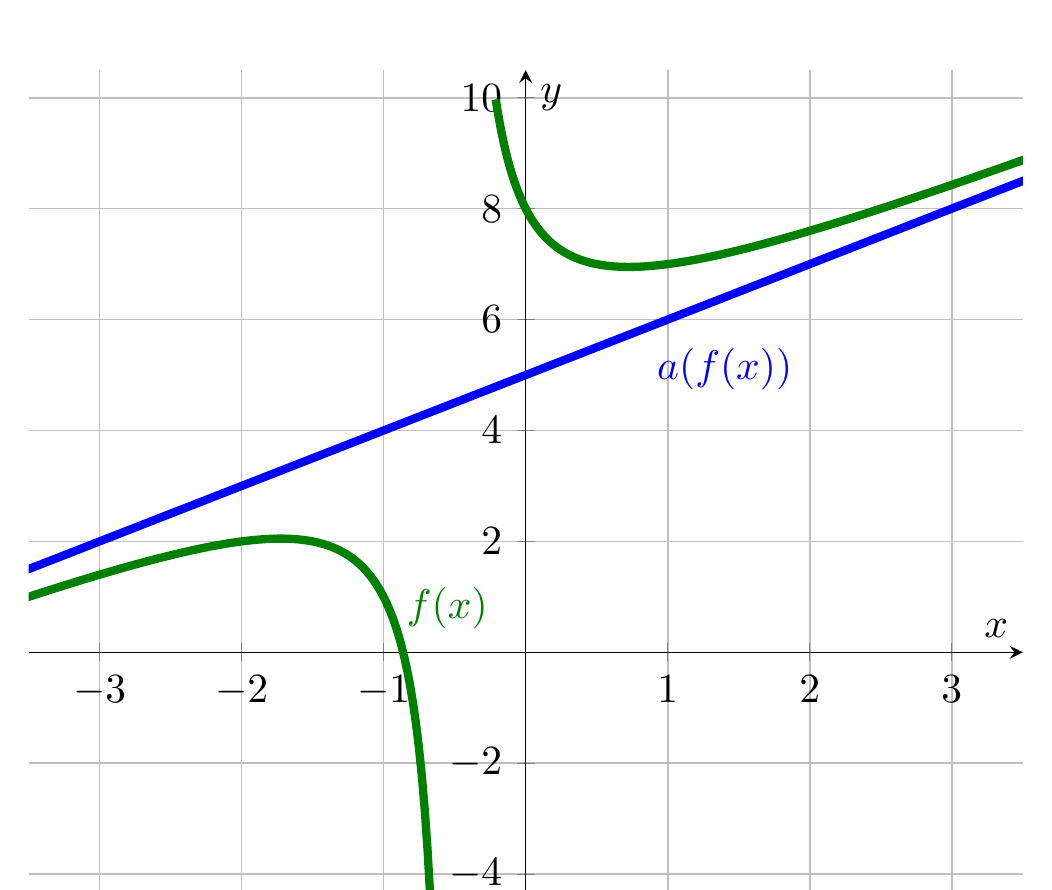
\begin{tikzpicture}[scale=1.5]
        \begin{axis}[
            axis lines=middle,
            samples=500,
            restrict x to domain=-4:4,
            restrict y to domain=-10:10,
            xlabel=$x$,
            ylabel=$y$,
            xmin=-3.5,
            xmax=3.5,
            ymin=-4.5,
            ymax=10.5,
            xmajorgrids=true,
            ymajorgrids=true,
        ]
        \foreach \COLOR/\EXPR/\LABEL/\POS/\LR in { 
            Green / { x+5+(3/(2*x+1)) } / $f(x)$ / 0.2 / right,
            Blue / {x+5} / $a(f(x))$ / 0.6 / below right
        } 
        {\edef\temp{
            \noexpand\addplot[line width=2pt,color=\COLOR]{\EXPR}
            node[\LR,pos=\POS]{\LABEL};
        }\temp} 
        \end{axis}
    \end{tikzpicture}
\end{center}
    \pagebreak

    \subsection{}
    \begin{tcolorbox}
        Určete Taylorův polynom 2. řádu funkce $f$ se středem v bodě $x_0$, je-li
        $$ f(x) \coloneq \sin{x} + \cos{x} + \tan{x},\ x_0 = 0 . $$
    \end{tcolorbox}
    %%% Uses the table of data generated by python 
Let's try direct substituting $x = 0$.

\begin{align}
    \lim_{x \rightarrow 0}&\frac{x^{2019} + \sin{(2019x)}}{e^{2019x} - x - 1} \\
    &= \frac{0^{2019} + \sin{(2019(0))}}{e^{2019(0)} - 0 - 1} \\
    &= \frac{\sin{0}}{e^{0} - 1} = \frac{0}{0}
\end{align}

We get division by zero which is undefined, so we must go
a different route. Let's try $L'H\hat{o}pital's$ rule.

 \begin{align}
    \lim_{x \rightarrow 0}&
    \frac{x^{2019} + \sin{(2019x)}}{e^{2019x} - x - 1} \\
    &=\frac{(x^{2019} + \sin{(2019x)})'}{(e^{2019x} - x - 1)'} \\
    &=\frac{2019x^{2018} + 2019\cos{(2019x)}}{2019e^{2019x} - 1} \\
    &=\frac{2019(0)^{2018} + 2019\cos{(2019(0))}}{2019e^{2019(0)} - 1} \\
    &=\frac{2019\cos{(0)}}{2019e^{0} - 1} =\frac{2019}{2018}
\end{align}

The result of limit $\Lim{x \rightarrow 0} \frac{x^{2019} + \sin{(2019x)}}
{e^{2019x} - x - 1}$ equals to $\frac{2019}{2018}$. 

\begin{center}
    \textit{Graph of function $f(x) \coloneq 
    \frac{x^{2019} + \sin{(2019x)}}{e^{2019x} - x - 1}$}

    \begin{tikzpicture}[scale=1.0]
        \begin{axis}[
            axis lines=middle,
            xlabel=$x$,
            ylabel=$y$,
            xmin=-0.007,
            xmax=0.007,
            ymin=-1.2,
            ymax=1.7,
            xmajorgrids=true,
            ymajorgrids=true,
            raw gnuplot,
        ]
        \foreach \COLOR/\PATH/\LR/\POS/\LABEL in {
            Green /{tables/table_1/plot_data.txt}/ right / 0.9 / {$f(x)$}
        } {
            \edef\temp{
                \noexpand\addplot[line width=2pt, color=\COLOR] 
                table[x index=0, y index=1]{\PATH}
                node[\LR,pos=\POS]{\LABEL};
            }
            \temp
        }
        \node (src) at (axis cs: {2*10^(-3)},1) {$(0,\frac{2019}{2018})$};
        \node (dest) at (axis cs: 0,{2019/2018}) {\textbullet};
        \draw[line width=1.2pt, ->, shorten >= -6pt, shorten <= -4pt](src)--(dest);
        \end{axis}
    \end{tikzpicture}
\end{center}

    \pagebreak

    \subsection{}
    \begin{tcolorbox}
        Vypočtěte
        $$ \int (2x + 3)e^x \diff{x} . $$
    \end{tcolorbox}
    I will use the per partes becuase 
I don't see how the sub-method will 
help me here.

\begin{center}
    \textit{Per partes method}
    $$ \int uv' = uv - \int vu' $$
\end{center}

The \textit{per partes} method is derived 
from the product rule in derivation ($(uv)' = u'v + uv'$).

\[
\begin{aligned}
    \text{Výběr funkce $f$:} & \quad f(x) = (2x + 3) \rightarrow f'(x) = 2 \\
    \text{Výběr funkce $g$:} & \quad g'(x) = e^x \rightarrow g(x) = e^x  \\
\end{aligned}
\]

\begin{align}
    \int &(2x + 3)e^x \diff{x} =\\
    &= (2x+3)e^x - 2\int e^x \diff{x} =\\
    &= (2x+3)e^x - 2e^x = \\
    &= e^x(2x + 1) + C 
\end{align}

    \pagebreak

    \subsection{}
    \begin{tcolorbox}
        Vypočtěte
        $$ \int_{0}^{\frac{\pi}{2}} \sin^3{x}\cos^2{x} \diff{x} . $$
    \end{tcolorbox}
    \qs{Vypočtěte limitu}{$$
    \lim_{\ntoinf} \cos(2\pi n)
$$}

\begin{align}
    \lim_{\ntoinf} \cos(2 \pi n) = 1
\end{align}

\pagebreak

    \pagebreak

    \subsection{}
    \begin{tcolorbox}
        finish
    \end{tcolorbox}

\end{document}
